% =============================================================================
% Appendix F: Wall-Clock Efficiency
% =============================================================================
\section{Wall-Clock Efficiency}\label{sec:wallclock}

\begin{figure}[h]
\centering
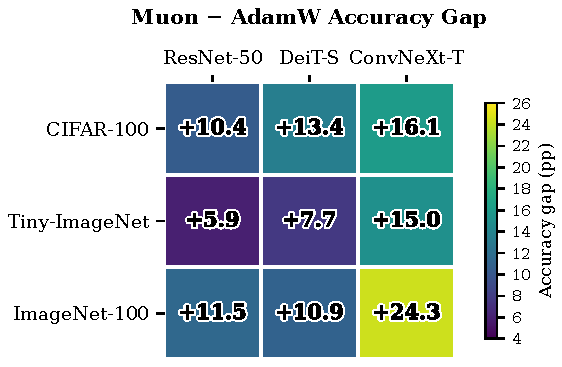
\includegraphics[width=0.42\textwidth]{figures/fig1_spectral_gap_heatmap.pdf}
\caption{Spectral--AdamW accuracy gap (pp) at 20 epochs. ConvNeXt-T consistently exhibits the largest gap ($+15.0$--$+24.3$\,pp); all gaps are positive across the full $3\times3$ matrix.}
\label{fig:gap_heatmap}
\end{figure}


\begin{table}[h]
\centering
\caption{Per-epoch wall-clock time (seconds) for 20-epoch training runs on a single RTX 5090 GPU.}
\label{tab:wallclock}
\small
\begin{tabular}{llcccc}
\toprule
Dataset & Architecture & Muon (s) & AdamW (s) & SGD (s) & Muon Overhead \\
\midrule
\multirow{3}{*}{CIFAR-100}
 & ResNet-50  & 58.8  & 53.4  & 53.2  & +10.1\% \\
 & DeiT-S     & 55.4  & 45.6  & 45.2  & +21.5\% \\
 & ConvNeXt-T & 116.8 & 106.9 & 107.1 & +9.3\%  \\
\midrule
\multirow{3}{*}{Tiny-ImageNet}
 & ResNet-50  & 118.2 & 99.5  & 96.5  & +18.8\% \\
 & DeiT-S     & 98.6  & 88.0  & 87.3  & +12.0\% \\
 & ConvNeXt-T & 219.2 & 208.2 & 205.6 & +5.3\%  \\
\midrule
\multirow{3}{*}{ImageNet-100}
 & ResNet-50  & 74.2  & 68.5  & 68.4  & +8.3\%  \\
 & DeiT-S     & 69.4  & 81.4$^\dagger$  & ---   & ---     \\
 & ConvNeXt-T & 134.4 & 122.5 & 123.6 & +9.7\%  \\
\bottomrule
\end{tabular}
\vspace{0.3em}
\par\noindent\footnotesize{Muon Overhead is computed relative to AdamW. $\dagger$\,DeiT-S AdamW on IN100 used a different batch configuration, making the timing comparison unreliable; IN100 DeiT-S SGD log was not found.}
\end{table}

\paragraph{Computational overhead of Newton-Schulz iteration.}
Muon's per-step cost exceeds AdamW by 5--22\% depending on architecture and dataset, attributable to the Newton-Schulz iteration used to approximate the matrix sign function for spectral-norm steepest descent. The overhead is largest on DeiT-S/CIFAR-100 (+21.5\%) where the parameter matrices are relatively small and the Newton-Schulz iterations dominate; it is smallest on ConvNeXt-T/Tiny-ImageNet (+5.3\%) where forward/backward pass computation amortizes the optimizer cost. SGD and AdamW have near-identical per-epoch times across all configurations, confirming that the overhead is specific to Muon's spectral decomposition.

\paragraph{Wall-clock break-even analysis.}
Despite 7--19\% per-epoch overhead from Newton-Schulz iterations, Muon reaches AdamW's final accuracy in far fewer epochs, yielding net wall-clock savings in every configuration tested (Table~\ref{tab:wallclock_breakeven}).
The advantage compounds with longer training horizons: median speedup rises from $2.3\times$ (20 epochs) to $8.6\times$ (50 epochs), because AdamW's marginal gains plateau while Muon converges early.
In no experiment does AdamW reach Muon's final accuracy within the allotted budget.

\begin{table}[h]
\centering
\caption{Wall-clock break-even analysis. \emph{Iso-accuracy target} is AdamW's final accuracy for each configuration; \emph{Muon ep} and \emph{AdamW ep} are the first epoch at which each optimizer reaches that target. Wall-clock speedup accounts for Muon's per-epoch overhead.}
\label{tab:wallclock_breakeven}
\small
\begin{tabular}{ll cc cc cc}
\toprule
 & & \multicolumn{2}{c}{Time/epoch (s)} & \multicolumn{2}{c}{Epochs to iso-acc} & \multicolumn{2}{c}{Speedup} \\
\cmidrule(lr){3-4} \cmidrule(lr){5-6} \cmidrule(lr){7-8}
Setting & Architecture & Muon & AdamW & Muon & AdamW & Epoch & Wall \\
\midrule
\multirow{3}{*}{\shortstack[l]{TIN\\20\,ep}}
 & ResNet-50  & 118.0 & 99.4  & 8  & 19 & $2.4\times$ & $2.0\times$  \\
 & ConvNeXt-T & 226.8 & 206.7 & 2  & 17 & $8.5\times$ & $7.6\times$  \\
 & DeiT-S     & 129.6 & 87.9  & 4  & 20 & $5.0\times$ & $2.3\times$  \\
\midrule
\multirow{3}{*}{\shortstack[l]{C100\\50\,ep}}
 & ResNet-50  & 59.4  & 51.8  & 11 & 49 & $4.5\times$ & $3.4\times$  \\
 & ConvNeXt-T & 109.5 & 102.4 & 3  & 49 & $16.3\times$ & $15.1\times$ \\
 & DeiT-S     & 54.6  & 47.1  & 5  & 50 & $10.0\times$ & $8.6\times$  \\
\bottomrule
\end{tabular}
\vspace{0.3em}
\par\noindent\footnotesize{C100 = CIFAR-100, TIN = Tiny-ImageNet. TIN 20\,ep uses seeds 1, 2; C100 50\,ep uses seed 2.}
\end{table}



% =============================================================================
% Appendix G: Alternative Spectral Optimizers
% =============================================================================
\section{Alternative Spectral Optimizers}\label{sec:alt_spectral}

\begin{table}[h]
\centering
\caption{Comparison of spectral optimizers on CIFAR-100 (20 epochs). Multi-seed means ($\pm$ std) reported where available; ConvNeXt-T SGD is single-seed (seed\,=\,42).}
\label{tab:spectral_comparison}
\small
\begin{tabular}{llcccc}
\toprule
 & & \multicolumn{4}{c}{Validation Accuracy (\%)} \\
\cmidrule(lr){3-6}
Architecture & & SOAP & Shampoo & Muon & AdamW \\
\midrule
ResNet-50  & & 77.28{\scriptsize$\pm$0.20} & 78.25{\scriptsize$\pm$0.18} & 76.88{\scriptsize$\pm$0.27} & 67.85{\scriptsize$\pm$0.17} \\
DeiT-S     & & 65.45{\scriptsize$\pm$0.18} & 63.53{\scriptsize$\pm$0.05} & 62.67{\scriptsize$\pm$0.41} & 52.33{\scriptsize$\pm$0.34} \\
ConvNeXt-T & & 74.40{\scriptsize$\pm$0.43} & 70.57{\scriptsize$\pm$0.29} & 74.62{\scriptsize$\pm$0.15} & 58.54{\scriptsize$\pm$2.17} \\
\bottomrule
\end{tabular}
\vspace{0.3em}
\par\noindent\footnotesize{Muon and AdamW values are multi-seed means ($\pm$ std), consistent with Table~\ref{tab:main_results}. SOAP is 3-seed; Shampoo is 3-seed on all architectures ($\text{lr}{=}7{\times}10^{-3}$ on ConvNeXt-T). All optimizers use per-architecture tuned learning rates from 5-epoch sweeps; Shampoo learning rates were refined via extended sweeps (Appendix~\ref{sec:hyperparams}).}
\end{table}

% =============================================================================
% Appendix I: Architecture Coverage Rationale
% =============================================================================
% =============================================================================
% Appendix: Layer-wise Spectral Analysis (Full)
% =============================================================================
\section{Layer-wise Spectral Analysis and Training Stability}\label{sec:spectral_analysis_full}

To localize where Muon's advantage arises within the network, we apply the weight swap protocol and spectral correlation analysis (Section~\ref{sec:method}) to CIFAR-100 models.

\paragraph{Weight Swap Results.}
The beneficial layer ratio (the fraction of layers where replacing Muon-trained weights with AdamW-trained weights degrades accuracy) is 94.3\% (50/53 layers) for ResNet-50 and 51.7\% (46/89 parameter groups) for DeiT-S.
Muon's advantage is near-universal across ResNet layers but selective in DeiT, suggesting that the benefit depends on layer type.

\paragraph{Spectral Divergence Correlations.}
Using checkpoints trained at independently selected optimal learning rates (Muon $\eta{=}0.02$, AdamW $\eta{=}10^{-3}$ for ResNet-50; Muon $\eta{=}0.003$, AdamW $\eta{=}10^{-4}$ for DeiT-S), we compute the Spearman rank correlation between per-layer stable rank divergence $\Delta \mathrm{sr}_l$ and per-layer Muon benefit $\Delta a_l$.
For ResNet-50, $\rho = +0.58$ ($p = 3.6 \times 10^{-6}$, after BN recalibration; original $\rho = +0.53$ before recalibration): layers where Muon and AdamW diverge most in stable rank tend to be the layers where Muon contributes the most.
For DeiT-S, no significant correlation is observed ($\rho \approx 0$, n.s.), indicating that the relationship between stable rank divergence and per-layer benefit is architecture-dependent.

\paragraph{Training Stability Across Seeds.}

\begin{figure}[h]
\centering
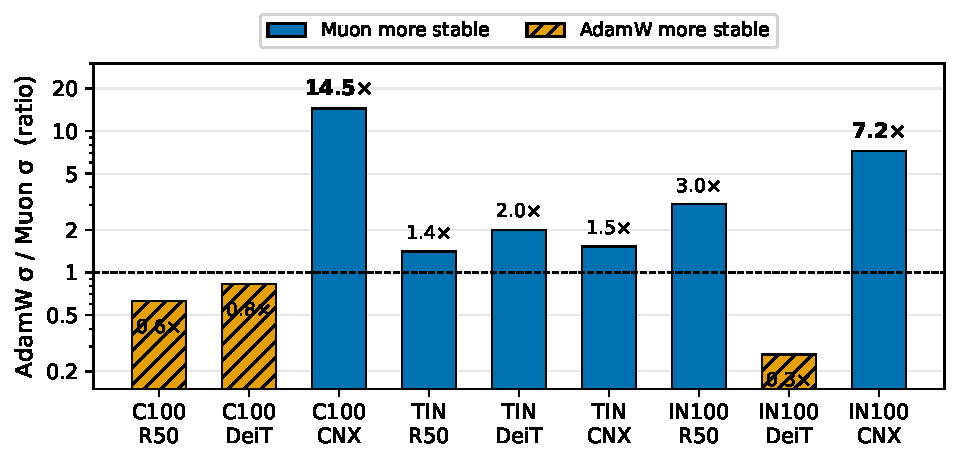
\includegraphics[width=\textwidth]{figures/fig3_stability.pdf}
\caption{Cross-seed standard deviation ($\sigma$) for Muon vs AdamW across all nine settings. Muon exhibits lower variance on 6/9 configurations; the stability advantage is architecture-dependent.}
\label{fig:stability}
\end{figure}

Cross-seed variance is architecture-dependent (Figure~\ref{fig:stability}): Muon shows substantially lower variance on convolutional architectures ($\sigma{=}0.15$ vs.\ $2.17$ on ConvNeXt-T/CIFAR-100), but AdamW is more stable on DeiT-S/ImageNet-100 ($\sigma{=}0.10$ vs.\ $0.38$).
Where Muon's variance reduction exceeds $7\times$ (ConvNeXt-T), fewer seeds suffice for reliable estimates.

% =============================================================================
% Appendix: Metric Robustness
% =============================================================================
\section{Metric Robustness}\label{sec:metric_robustness}

The architecture-dependent correlation pattern reported in Section~\ref{sec:spectral_analysis} is verified across alternative spectral metrics. We compute the Spearman correlation between per-layer Muon benefit $\Delta a_l$ and three alternative divergence measures:

\begin{table}[h]
\centering
\caption{Spearman $\rho$ between per-layer divergence and Muon benefit under three spectral metrics. The positive correlation on ResNet-50 is consistent across all metrics; DeiT-S shows no significant pattern ($\rho \approx 0$, n.s.).}
\label{tab:metric_robustness}
\small
\begin{tabular}{@{}lcccc@{}}
\toprule
Metric & \multicolumn{2}{c}{ResNet-50} & \multicolumn{2}{c}{DeiT-S} \\
\cmidrule(lr){2-3} \cmidrule(lr){4-5}
 & $\rho$ & $p$ & $\rho$ & $p$ \\
\midrule
$\Delta\mathrm{sr}_l$ (stable rank) & $+0.58$ & $3.6{\times}10^{-6}$ & $\approx 0$ & n.s. \\
FCSB margin & $+0.40$ & ${<}0.01$ & $\approx 0$ & n.s. \\
$\Delta\mathrm{er}_l$ (effective rank) & $+0.43$ & ${<}0.01$ & $\approx 0$ & n.s. \\
\bottomrule
\end{tabular}
\end{table}

All three metrics yield positive correlations on ResNet-50; DeiT-S shows no significant correlation under any metric.
We adopt stable rank as the primary metric for its favorable analytical properties: it is bounded, well-defined for rank-deficient matrices, and requires no architecture-specific normalization.

% =============================================================================
% Appendix: Normalization Swap Details
% =============================================================================
\section{Normalization Swap Implementation}\label{sec:normswap_details}

We replace all BatchNorm2d layers in ResNet-50 with GroupNorm(1, $C$), where $C$ is the number of channels.
GroupNorm with a single group computes statistics over all spatial and channel dimensions of each sample independently, making it equivalent to LayerNorm applied to convolutional feature maps~\cite{wu2018group}.
This substitution replaces 53 BatchNorm layers; all other architecture parameters, hyperparameters, and the training protocol remain identical to the standard ResNet-50 experiments (Section~\ref{sec:experimental_setup}).

% =============================================================================
% Appendix: Ablation Details
% =============================================================================
\section{Parameter Grouping Ablation Details}\label{sec:ablation_details}

The two-group AdamW ablation mirrors Muon's parameter routing exactly: 53 two-dimensional weight matrices ($23.45$M parameters, $\text{lr}{=}10^{-3}$) and 108 one-dimensional parameters ($0.26$M parameters, $\text{lr}{=}3{\times}10^{-4}$), with AdamW applied to both groups.
On ResNet-50 (CIFAR-100), two-group AdamW achieves $66.36 \pm 0.40\%$ ($n{=}3$, seeds 42/2/3), comparable to single-group AdamW ($67.85 \pm 0.17\%$) and far below Muon ($76.88 \pm 0.27\%$).
On ConvNeXt-T, two-group AdamW similarly matches standard AdamW ($59.44 \pm 0.28\%$ vs.\ $58.54 \pm 2.17\%$) while Muon maintains a $+15.2$\,pp advantage ($74.62 \pm 0.15\%$).
On DeiT-S, two-group AdamW degrades catastrophically to $30.08\%$ ($-22.3$\,pp vs.\ standard AdamW, single seed), as the reduced learning rate for 1D parameters (104/152 tensors in DeiT-S) severely undertrained LayerNorm parameters.
% =============================================================================
% Appendix: Additional Optimizer Comparisons
% =============================================================================
\section{Additional Optimizer Comparisons}\label{sec:additional_optimizers}

We evaluated Lion~\cite{chen2024lion} as a representative of sign-based optimizers to verify that the spectral optimizer class's advantage is not shared by all non-Adam methods.
On ResNet-50/CIFAR-100, Lion achieves $69.42\%$ (vs.\ AdamW $67.85\%$, $+1.57$\,pp), far below the spectral optimizer class ($+9$--$+10$\,pp over AdamW), confirming that the advantage is specific to spectral preconditioning rather than a general property of non-diagonal methods.
Other recent optimizers, such as Sophia~\cite{liu2024sophia} (diagonal Hessian clipping), Prodigy~\cite{mishchenko2024prodigy} (learning-rate-free estimation), GaLore~\cite{zhao2024galore} (low-rank gradient projection), target computational cost or tuning difficulty rather than architecture robustness, making them complementary to rather than competitors of spectral methods.
A comprehensive comparison with these methods is left to future work.

% =============================================================================
% Appendix I: Architecture Coverage Rationale
% =============================================================================
\section{Architecture Coverage in Supplementary Experiments}\label{sec:arch_coverage}

The extended experiments in Appendix~\ref{sec:alt_spectral} focus on ResNet-50 and ConvNeXt-T rather than all three architectures from the main experiments. These two architectures represent the extremes of the normalization spectrum that drives Muon's variable effectiveness: ResNet-50 uses BatchNorm, where Muon's spectral updates interact with the implicit conditioning provided by BN; ConvNeXt-T uses LayerNorm, where the Muon--AdamW gap is largest (up to +24.30\,pp on IN100 at 20 epochs). DeiT-S, which also uses LayerNorm but in a pure self-attention architecture, exhibits intermediate gap magnitudes and is already thoroughly characterized across three datasets, three seed replicates, and two training horizons (20 and 50 epochs) in the main paper. Including DeiT-S in the supplementary experiments would add six additional training runs without meaningfully extending the analysis beyond the BN--LN axis already captured by the ResNet-50/ConvNeXt-T pair.

\section{Corruption Robustness}\label{sec:corruption_robustness}

We evaluate corruption robustness on CIFAR-100-C~\cite{hendrycks2019benchmarking}, which applies 19 corruption types at 5 severity levels to the CIFAR-100 test set. We report mean corruption error (mCE), normalized so that same-architecture, same-normalization AdamW = 100\%; lower is better.

\begin{table}[h]
\centering
\caption{Corruption robustness on CIFAR-100-C. mCE ($\downarrow$ is better) normalized so same-normalization AdamW = 100\%. Retention = corruption accuracy\,/\,clean accuracy, measuring inherent robustness independent of clean performance level. mCE is computed over the standard 15 corruption types \citep{hendrycks2019benchmarking}.}
\label{tab:corruption_robustness}
\small
\begin{tabular}{llcccc}
\toprule
Architecture & Optimizer & Clean Acc (\%) & Corr Acc (\%) & mCE (\%) & Retention (\%) \\
\midrule
\multirow{4}{*}{ResNet-50 (BN)} & SOAP & 77.28 & 22.74 & \textbf{98.6} & 29.4 \\
 & Shampoo & 78.25 & 21.94 & 99.8 & 28.0 \\
 & AdamW & 67.85 & 22.40 & 100.0 & 33.0 \\
 & Muon & 76.88 & 21.59 & 100.5 & 28.1 \\
\midrule
\multirow{2}{*}{ResNet-50 (LN)} & Muon & 78.52 & 27.44 & \textbf{92.6} & 34.9 \\
 & AdamW & 50.51 & 22.93 & 100.0 & 45.4 \\
\midrule
\multirow{4}{*}{ConvNeXt-T} & Muon & 74.59 & 26.66 & \textbf{94.6}{\scriptsize$\pm$0.5} & 35.7 \\
 & SOAP & 74.40 & 26.23 & 95.1{\scriptsize$\pm$0.1} & 35.3 \\
 & AdamW & 59.81 & 21.12 & 100.0 & 35.3 \\
 & Shampoo & 70.57 & 23.55 & 98.1{\scriptsize$\pm$0.4} & 33.4 \\
\midrule
\multirow{4}{*}{DeiT-S} & Muon$^\ddagger$ & 62.26 & 21.65 & 98.6 & 34.8 \\
 & SOAP & 65.45 & 21.47 & \textbf{98.3} & 32.8 \\
 & AdamW & 52.33 & 20.89 & 100.0 & 39.9 \\
 & Shampoo & 63.53 & 18.77 & 102.6 & 29.5 \\
\midrule
\multirow{5}{*}{ResNet-50 (GN32)} & Muon & 78.20 & 28.75 & \textbf{90.0} & 36.8 \\
 & SOAP & 75.52 & 27.88 & 91.3 & 36.9 \\
 & Shampoo & 74.79 & 26.96 & 92.6 & 36.0 \\
 & AdamW & 55.73 & 22.58 & 100.0 & 40.5 \\
 & SGD & 23.90 & 14.36 & 112.9 & 60.1 \\
\bottomrule
\end{tabular}
\vspace{0.3em}
\par\noindent\footnotesize{$^\ddagger$\,DeiT-S Muon: corrected using seed=2 baseline checkpoint (clean acc 62.26\%); previous report (mCE 89.2\%) used enhanced checkpoint.}
\par\noindent\footnotesize{ConvNeXt-T mCE: multi-seed means ($n$\,=\,3 for Muon/SOAP, $n$\,=\,2 for Shampoo). Shampoo's lower clean accuracy (70.4\% vs 74.5\%) may partially confound the mCE comparison through floor effects on noise corruptions.}
\par\noindent\footnotesize{Spectral preconditioning method: Muon and SOAP use Newton--Schulz iteration; Shampoo uses Kronecker factorization.}
\end{table}

Muon achieves the lowest mCE on two of four architecture configurations (ConvNeXt-T: 94.6\%, ResNet-50-LN: 92.6\%), with the robustness advantage most pronounced on layer-normalized architectures. On DeiT-S, the corrected Muon mCE (98.6\%, using seed=2 baseline checkpoint with 62.26\% clean accuracy) is marginally above SOAP (98.3\%), indicating that the previously reported advantage was an artifact of using an enhanced checkpoint. On ResNet-50 with BatchNorm, differences among optimizers are marginal (mCE 98.6--100.5\%), consistent with BatchNorm's known loss-landscape smoothing effect. Shampoo underperforms AdamW on DeiT-S (mCE 102.6\%) and performs near-baseline on ResNet-50-BN (99.8\%), but shows moderate improvement on ConvNeXt-T (98.1\%) under multi-seed evaluation. Category-level analysis reveals that Muon's advantage concentrates in weather and digital corruptions (brightness, saturate, snow, frost, spatter), while noise corruptions (Gaussian, shot, impulse) show smaller inter-optimizer differences.

\paragraph{Dose-response pattern in corruption robustness.}
The GN(32) configuration extends the dose-response pattern observed in clean accuracy (Section~\ref{sec:norm_swap}) to corruption robustness. Under GN(32), all three spectral optimizers improve mean corruption accuracy by 5--7\,pp relative to their BN counterparts (Muon: $+7.2$\,pp, SOAP: $+5.1$\,pp, Shampoo: $+5.0$\,pp), while AdamW remains flat ($+0.2$\,pp). SGD under GN(32) degrades to 14.36\% mean corruption accuracy (mCE 112.9\%), an 8.2\,pp drop below GN(32) AdamW, mirroring the clean-accuracy collapse observed in the normalization-swap experiment. This three-way divergence (spectral methods improve, AdamW holds steady, SGD degrades) constitutes a dose-response pattern: as normalization smoothing is reduced from BN to GN(32), the optimizer's capacity for spectral preconditioning determines whether it can compensate for the lost implicit conditioning, in corruption robustness as in clean accuracy.

\subsection{Spectral Divergence Profile}
\label{app:spectral-divergence}

We formalize the \emph{stable rank divergence} $\rho$ as a post-hoc diagnostic
for whether a spectral optimizer structurally modifies the weight spectrum.

\paragraph{Definition.}
For a trained model with weight matrices $\{W_l\}_{l=1}^L$, the \emph{stable rank} of layer $l$ is
\begin{equation}
  \mathrm{SR}(W_l) \;=\; \frac{\|W_l\|_F^2}{\|W_l\|_2^2}\,,
\end{equation}
where $\|\cdot\|_F$ and $\|\cdot\|_2$ denote the Frobenius and spectral norms.
Given a spectral optimizer $\mathcal{S}$ and a baseline $\mathcal{B}$ (AdamW), the
\emph{stable rank divergence} is
\begin{equation}
  \rho(\mathcal{S}, \mathcal{B}) \;=\; \frac{1}{L}\sum_{l=1}^{L}
    \frac{\mathrm{SR}_{\mathcal{S}}(W_l) - \mathrm{SR}_{\mathcal{B}}(W_l)}
         {\mathrm{SR}_{\mathcal{B}}(W_l)}\,.
  \label{eq:rho}
\end{equation}
A positive $\rho$ indicates that the spectral optimizer distributes singular value
mass more uniformly than AdamW (higher effective rank).

\paragraph{Empirical findings.}
We compute $\rho$ from best-checkpoint weights across three architecture configurations
(Table~\ref{tab:rho}).
All spectral optimizers yield $\rho > 0$ ($n=7/7$), confirming that they
structurally increase the effective dimensionality of learned representations.

\begin{table}[h]
\centering
\small
\caption{Stable rank divergence $\rho$ and accuracy advantage $\Delta\mathrm{acc}$
over AdamW baseline. All checkpoints are best validation accuracy (seed 42).}
\label{tab:rho}
\begin{tabular}{llrr}
\toprule
Architecture & Optimizer & $\rho$ & $\Delta$acc (\%) \\
\midrule
ResNet-50 (BN) & Muon    & 2.10 & $+$8.89  \\
               & SOAP    & 3.92 & $+$9.34  \\
               & Shampoo & 3.44 & $+$10.03 \\
\midrule
ResNet-50 (LN) & Muon    & 6.94 & $+$26.37 \\
\midrule
ConvNeXt-T\textsuperscript{\dag}
               & Muon    & 4.53 & $+$11.78 \\
               & SOAP    & 7.79 & $+$8.46  \\
               & Shampoo & 8.49 & $+$4.67  \\
\bottomrule
\multicolumn{4}{l}{\footnotesize \textsuperscript{\dag}Evaluated under enhanced training recipe.}
\end{tabular}
\end{table}

\paragraph{Within-architecture ranking.}
We observe a negative \emph{observational} correlation between $\rho$ and
$\Delta\mathrm{acc}$ within each architecture: on both ResNet-50 (BN) and
ConvNeXt-T, the optimizer with the \emph{lowest} $\rho$ achieves the
\emph{highest} accuracy gain (Kendall $\tau = -1.0$ on ConvNeXt-T).
That is, the most effective spectral optimizers apply \emph{minimal} spectral
restructuring for maximal downstream improvement, rather than indiscriminately
flattening the singular value spectrum.

\paragraph{Normalization and spectral modification.}
Comparing ResNet-50 under BatchNorm vs.\ LayerNorm reveals that Muon's
$\rho$ increases from 2.10 (BN) to 6.94 (LN), a $3.3\times$ increase.
When BatchNorm's implicit spectral conditioning is removed, the optimizer must
perform substantially more spectral restructuring to maintain performance.
This is consistent with the dose-response pattern observed in
Section~\ref{sec:spectral_analysis}: spectral optimizers compensate for the loss of
normalization-induced regularization, and the magnitude of compensation scales
with the degree of normalization removal.

\paragraph{Limitations.}
This analysis reports observational correlations from CIFAR-100 scale
experiments (20 epoch budgets) and should not be interpreted causally.
The ResNet-50 (LN) AdamW baseline (51.9\%) reflects suboptimal hyperparameter
transfer rather than inherent optimizer failure, inflating the apparent
$\Delta\mathrm{acc}$.
Validating $\rho$ as a \emph{predictive} (rather than post-hoc) diagnostic
requires computing stable ranks from early-training checkpoints and testing
on larger-scale datasets, which we leave to future work.

\subsection{Tiny-ImageNet: SOAP and Shampoo Results}
\label{sec:tinyin_soap_shampoo}

Table~\ref{tab:tinyin_spectral} reports Tiny-ImageNet accuracy for all three spectral optimizers across architectures, complementing the CIFAR-100 results in the main text.

\begin{table}[h]
\centering
\caption{Tiny-ImageNet 20-epoch accuracy (\%) for spectral optimizers. The ranking Muon $>$ SOAP $>$ Shampoo holds on ResNet-50 and ConvNeXt-T. On DeiT-S, all three spectral optimizers cluster within 3.5\,pp, with SOAP slightly leading.}
\label{tab:tinyin_spectral}
\small
\begin{tabular}{lccc}
\toprule
Architecture & Muon & SOAP & Shampoo \\
\midrule
ResNet-50 & 62.66 & 61.48 & 57.99 \\
DeiT-S & 48.02 & 51.49 & 50.58 \\
ConvNeXt-T & 58.92 & 57.46 & 49.98 \\
\bottomrule
\end{tabular}
\end{table}

The ranking Muon $>$ SOAP $>$ Shampoo holds on ResNet-50 and ConvNeXt-T. On DeiT-S, all three spectral optimizers cluster within 3.5\,pp, with SOAP slightly leading, with the largest gap on ConvNeXt-T ($\Delta_{\text{Muon--Shampoo}} = 8.94$\,pp). This cross-dataset replication strengthens the Newton-Schulz vs.\ Kronecker distinction reported in Section~5.

\subsection{Early Convergence Speed on ImageNet-1K}
\label{sec:imagenet1k_convergence}

To assess scalability beyond CIFAR-100 and Tiny-ImageNet, we compare early training dynamics on ImageNet-1K (ResNet-50, single GPU).

\begin{table}[h]
\centering
\caption{ImageNet-1K early convergence comparison: Muon reaches AdamW's accuracy in $\sim$4$\times$ fewer epochs.}
\label{tab:in1k_convergence}
\small
\begin{tabular}{lcc}
\toprule
Milestone & Muon epoch & AdamW epoch \\
\midrule
$\sim$63.9\% val acc & 5 & 20 \\
$\sim$67.1\% val acc & 8 & 33 \\
\bottomrule
\end{tabular}
\end{table}

At epoch~5, Muon reaches 63.9\% top-1 accuracy, matching AdamW's epoch-20 accuracy---a 4$\times$ epoch speedup consistent with findings on smaller datasets (Table~\ref{tab:wallclock_breakeven}). At epoch~8, Muon achieves 67.1\%, which AdamW requires $\sim$33 epochs to match. These results suggest the spectral advantage persists at ImageNet scale.

\subsection{Per-Layer Attention Analysis in DeiT-S}
\label{sec:deit_attention}

To determine whether Muon's spectral advantage concentrates in attention or MLP layers, we decompose the per-layer analysis of DeiT-S into four weight components per transformer block. Table~\ref{tab:sr_by_component} reports the stable rank ratio (Muon/AdamW) averaged across layers~1--11.

\begin{table}[h]
\centering
\caption{Stable rank ratio (Muon/AdamW) by weight component in DeiT-S, averaged over layers 1--11.}
\label{tab:sr_by_component}
\small
\begin{tabular}{lcc}
\toprule
Component & Mean SR Ratio & Shape \\
\midrule
MLP fc1 (fan-out) & 4.18 & $384 \to 1536$ \\
Q/K/V projection (square) & 3.49 & $384 \to 384$ each \\
Output projection (square) & 2.17 & $384 \to 384$ \\
MLP fc2 (fan-in) & 1.68 & $1536 \to 384$ \\
\bottomrule
\end{tabular}
\end{table}

Muon's advantage does \emph{not} concentrate in attention layers: attention SR ratio ($2.83\times$) and MLP SR ratio ($2.93\times$) are comparable. The true driver is \emph{matrix geometry}: the fc1 fan-out layer ($4.18\times$) shows the strongest spectral divergence, followed by square matrices (QKV: $3.49\times$, proj: $2.17\times$), with fan-in (fc2: $1.68\times$) lowest. The SR ratio is primarily driven by the fc1 fan-out layer, consistent with Muon's Newton-like update acting more aggressively when the matrix has more room for rank expansion along the output dimension.

AdamW concentrates $2$--$3\times$ more energy in the top-5 singular values than Muon across all components (e.g., Q/K/V: Muon 4.65\% vs.\ AdamW 11.97\%), confirming that Muon produces more uniformly distributed singular value spectra regardless of functional role.

\begin{figure}[h]
    \centering
    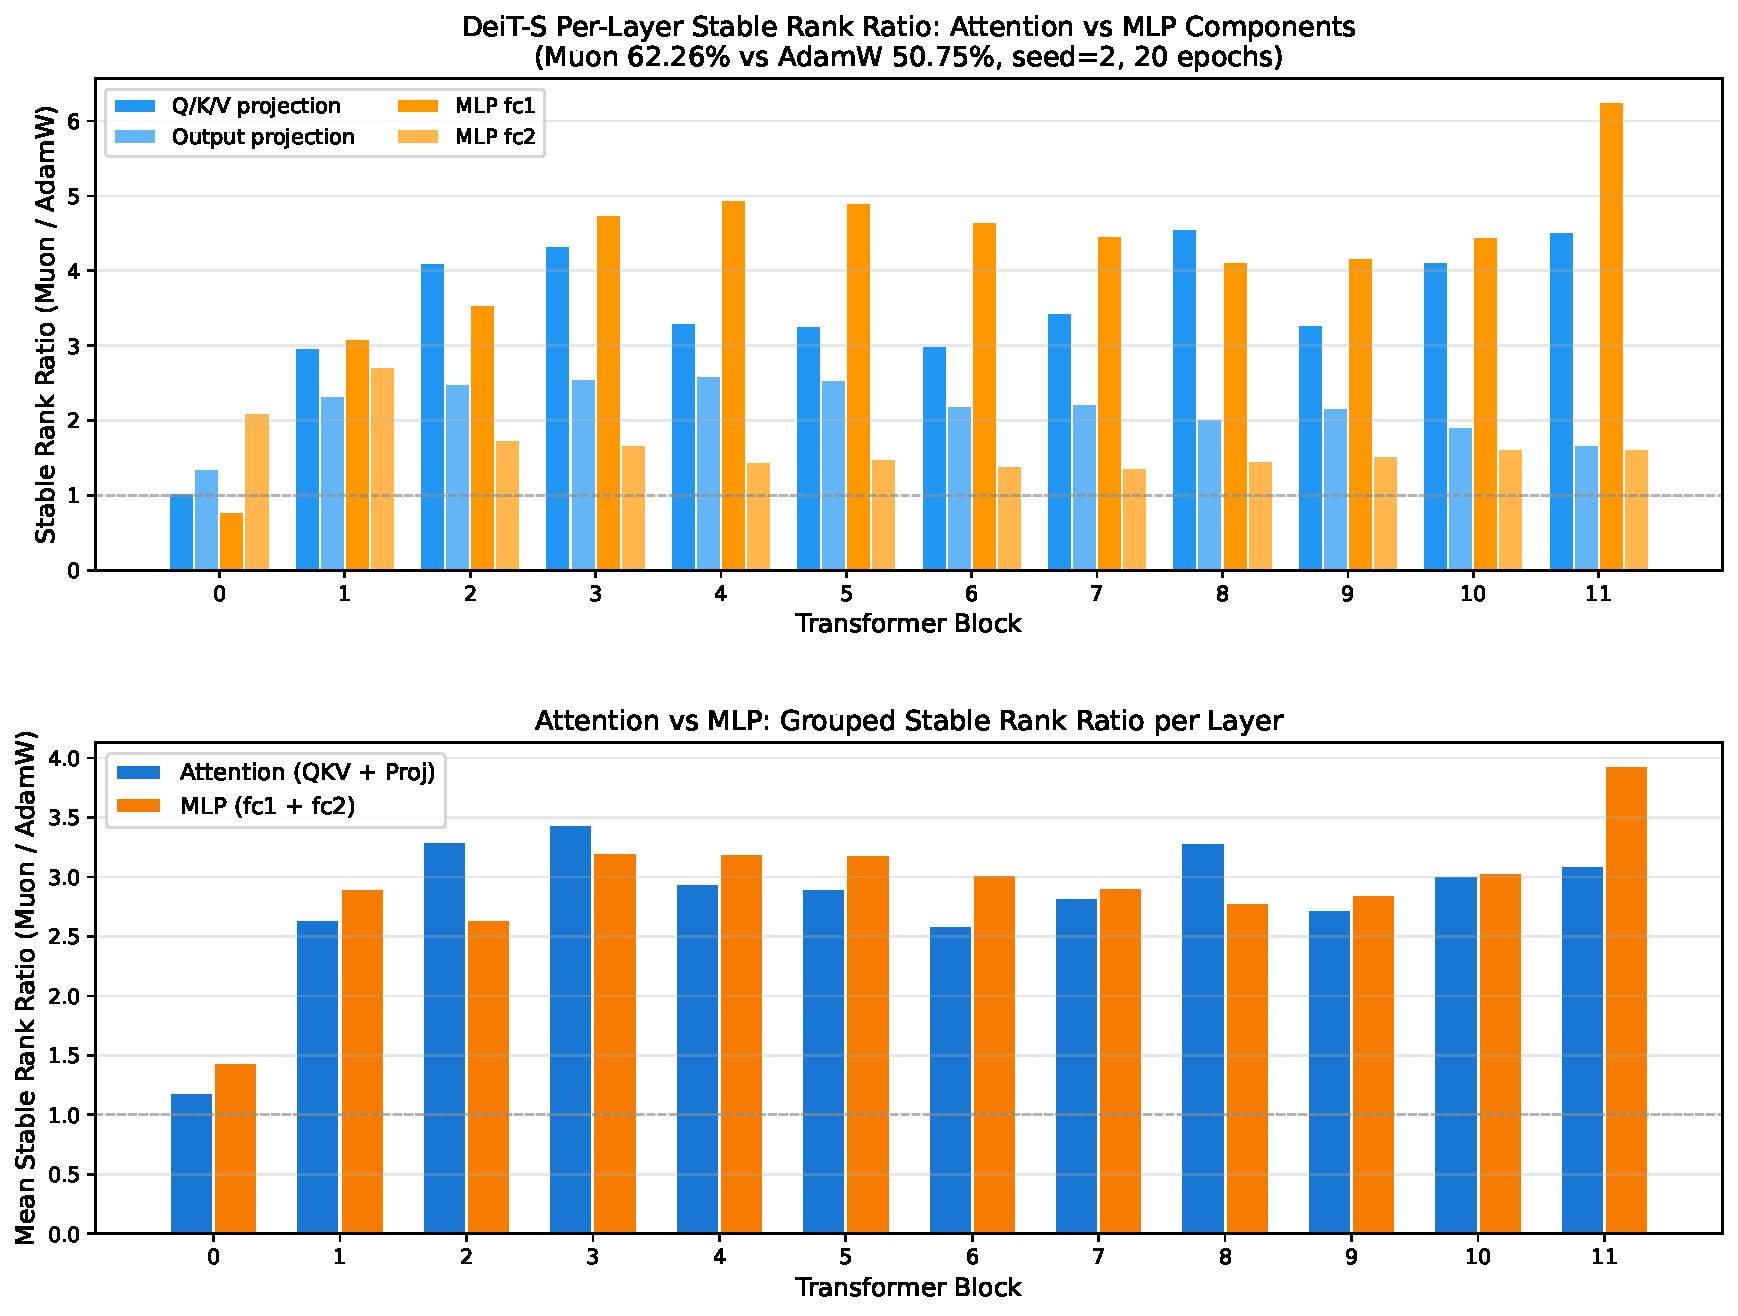
\includegraphics[width=\linewidth]{figures/deit_attention_spectral.pdf}
    \caption{Per-layer stable rank ratio (Muon/AdamW) in DeiT-S, decomposed by component. The spectral divergence is primarily driven by the fc1 fan-out layer rather than functional role (attention vs.\ MLP).}
    \label{fig:deit_attention_spectral}
\end{figure}


\medskip\noindent\textit{Note: Based on a single seed; multi-seed validation would strengthen layer-level patterns.}

